\chapter{Design \& Implementation}\label{sec:impl}

\section{Bitwidth analysis}
The analysis is a data flow analysis. The analysis attaches a $(int,boolean)$ tuple to every meaningful node. A node is considered meaningful is the node has a integer style mode. We will reference the first value as \emph{stable bits} and the second bit as \emph{is positive}.

\paragraph{Bit representation}
The stable bits are indicating how many bits are stable, and therefore not used.
The second value of the tuple indicates if the value will ever reach negative numbers or not. And thus indicate at least one stable bit at the highest position. However, the second value is only meaningful for modes that allow signs.

\paragraph{Range representation}
There is also a second way of interpreting the two values. The stable bits can define a minimum and maximum range. The maximum number is reached if the stable bits are just always zero. If the mode is signed and the node is not positive, then the minimum number is reached by assuming all stable bits are one. Otherwise the minimum range is 0. We can define the following min max definitions for the ranges:

$
max_{bitwidth}(x)=
\left\{
\begin{array}{l}2^{stable\_digits-1}-1\\2^{stable\_digits}-1\end{array}
\begin{array}{l} {mode.signed} \\ {Otherwise} \end{array}
\right.
$

$
min_{bitwidth}(x)=
\left\{
\begin{array}{l}2^{stable\_digits-1}\\0\end{array}
\begin{array}{l} {mode.signed and is_positive} \\ {Otherwise} \end{array}
\right.
$

\begin{figure}
	\centering
	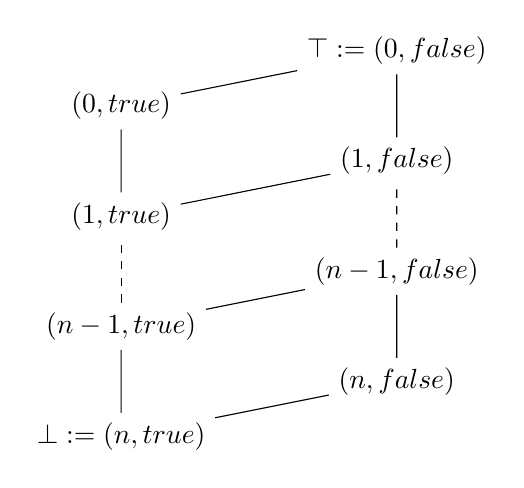
\begin{tikzpicture}[scale=.7]
		\node (np0) at(0,0) {$\bot := (n,true)$};
		\node (np1) at(0,2) {$(n-1,true)$};
		\node (np2) at(0,4) {$(1,true)$};
		\node (np3) at(0,6) {$(0,true)$};
		\node (p0) at(5,1) {$(n,false)$};
		\node (p1) at(5,3) {$(n-1,false)$};
		\node (p2) at(5,5) {$(1,false)$};
		\node (p3) at(5,7) {$\top := (0,false)$};
		\draw (np0) -- (p0) -- (p1) -- (np1) -- (np0);
		\draw (np2) -- (p2) -- (p3) -- (np3) -- (np2);
		\draw [dashed] (np1) -- (np2);
		\draw [dashed] (p1) -- (p2);
	\end{tikzpicture}
\caption{The definition of a upper bound compare node}
\label{fig:lattice}
\end{figure}

\paragraph{Analysis} The analysis works as a fixed point iteration. Therefore we use  \ref{fig:lattice} as lattice. The values of the lattice are representing the tuples from the analysis.

As a first step, we iterate over every single node and initialize the node with $\top$ and mark it as \textit{dirty}. If the node is constant, we calculate its bitwidth. Nodes with the opcodes \textit{Const}, \textit{Size} and \textit{Address} are considered constant.

The second step consists of recalculating every \textit{dirty} node in the graph. if $node.bitwidth < computed\_bitwidth$, the computed bitwidth is memorized as the new bitwidth of the node and every successor of the node is marked as dirty. The used rules for recalculating the nodes are described in REFERENCE TO TABLE %TODO.

\subsection{Value prediction}
In addition to the normal analysis results, the fixed point iteration can insert additional 
confirm nodes. Those confirm nodes help making the analysis more accurate.
First of all we need a few definitions for easier understanding:

\subparagraph{Definition: True / false Blocks}
A compare node in \libFIRM has always a relation, 2 operands and 2 blocks. One of the blocks is executed depending on if the criteria was meet or not. The block that is executed when it was meet, is called \emph{true-block} the other block is called \emph{false-block}. The structure is visualized in \ref{fig:compare_upper_bound}
\begin{figure}
	\centering
	\begin{tikzpicture}[scale=1.0, transform shape]
	\node[graph]{
		\begin{tikzpicture}[remember picture]
		\node[block] (startblock) {
			\begin{tikzpicture}
			\node[firm]    (predessors)       at (-1,3) {First};
			\node[firm]    (c2)       at ( 1,3) {Second};
			\node[firm]    (cmp)        at ( 0,2) {Cmp};
			\node[control] (cond)       at ( 0,1) {Cond};
			\node[control] (false)      at (-1,0) {Proj};
			\node[control] (true)       at ( 1,0) {Proj};
			
			\draw[dataDependency]    (cmp.120)     -- ++(0,0.1) -| (predessors);
			\draw[dataDependency]    (cmp.60)      -- ++(0,0.1) -| (c2);
			\draw[dataDependency]    (cond)        --              (cmp);
			\draw[controlDependency] (false.north) -- ++(0,0.1) -| (cond.240);
			\draw[controlDependency] (true.north)  -- ++(0,0.1) -| (cond.300);
			\end{tikzpicture}
		};
		\node[block, anchor=north east] (left) at ($(startblock.south) + (-1,-0.5)$) {
			\begin{tikzpicture}
			\node[const] (c0) at (0,0) {true-block};
			\end{tikzpicture}
		};
		\node[block, anchor=north west] (right) at ($(startblock.south) + (1,-0.5)$) {
			\begin{tikzpicture}
			\node[const] (c1) at (0,0) {false-block};
			\end{tikzpicture}
		};		
		% Control dependencies
		\begin{scope}[every path/.style = {controlDependency}]
			\draw (left.north)  -- ++(0,0.2) -| (false);
			\draw (right.north) -- ++(0,0.2) -| (true);
		\end{scope}
		
	\end{tikzpicture}
};
\end{tikzpicture}
\caption{The definition of a upper bound compare node}
\label{fig:compare_upper_bound}
\end{figure}


\subparagraph{Definition: Upper bounds}
A node defines a upper bound if the relation is < and the second operand is constant.\newline
A compare node is also defining a upper bound if it can be transformed into a construct that matches the definition. For example by switching the right and left nodes, while turning the relation.

\subparagraph{Definition: Predecessor in a certain block}
In the detection described later, we often need to find a predecessor that is placed in a certain block. Therefore we define:
\begin{center}
$\kappa(a, b) := \forall X \prec a \wedge X.block = b$ 
\end{center}

It will return every node that is located in \textit{b} and is a predecessor of \textit{a}.

\subparagraph{Definition: Constant dependencies}
While looking at C code we often see that add and mul nodes are used for calculating array addresses or addresses for struct access. Therefore one operant of the arithmetical operations is often constant. Knowing this a structure like FIXME %TODO
can be created. We define $\xi$ to explore the whole tree of one constant one not constant operants, and return us every node that was not constant.
\begin{center}
$\xi(a) := 
\left\{
	\begin{array}{l}
		a \cup \xi(c)\\ 
		\emptyset
	\end{array}
	\begin{array}{l}
		, \text{If there is only one not constant dependency \textit{c}} \\ 
		, \text{otherwise}.
	\end{array}
\right.$
\end{center}

If \textit{a} has only one not constant operant c, then $\xi$ returns the element a and $\xi(c)$. Otherwise it returns a empty set.

\paragraph{Upper bounds for block execution}
The values that are calculated in a node are (even if the fixed point iteration is not stable yet) possible values. The iteration starts at $\top$ and moves into the direction of $\bot$. This means that our range of possible values starts at something like $[0,0]$, moving towards $[n,-n]: n > 0 n <= max(mode)$ with each iteration. For a $\omega$ node this means that there can be a a recalculation, (new and old bitwidth is notated as the value range $\hat{x}$ and $x$) where the compare relation is true for $x$ but not anymore for  $\hat{x}$. This means that $\hat{x}$ is the upper bound for $\iota$. Thus we can insert a confirm node between every node $e \in \phi(\omega, \iota)$ and $\omega$.

\paragraph{Moving upper bounds backwards}
The confirms we have inserted between $\omega$ and its successors are not the only thing we can insert. We can also insert a confirm node between every $\phi(\xi(\omega), \iota)$. Important here is, the predecessors of $\omega$
Those confirms are then also inserted above conversation nodes, which is not possible using the normal construct insertion code provided by \libFIRM


\subsection{Difference to VRP}

There is already a analysis that is doing something similar, it is called value range propagation. The difference from VRP to BA is that in VRP each iteration is trying to predict the exact range after each operation. While BA tries to predict the unused bits after each operation. This little detail is mainly showing up in speed of the fixed point iteration, VRP converges way slower than BA. Details for this are given in the evaluation chapter \ref{sec:eval}.

\section{Stable Conversion nodes}
A conversion of a data word can result in two different results. First the bitwise representation stays the same. Second, the bitwise representation also gets mapped.
We call the first case \textit{Stable Conversion node}.

\paragraph{Finding stable conversion nodes}
Stable conversion nodes can be found using the bitwidth analysis. As described before, the analysis maps every node in the tree to a tuple. First number is the number of stable bits, which describes a upper bound for the numbers that will be written into the data word. The second number is a boolean flag and indicates if the number is going to be greater than 0 or not. If we now can see that the number range from the successor is the same as the one of the conversion node, then we can declare the conversion as stable.

\paragraph{Removing conversion nodes}
In case we found a stable conversion node, then we can say that this node only exists for syntax rules, there is no semantical value in them. Removing those nodes also has the advantage of helping other analysis. The confirm insertion algorithm of \libFIRM is searching for assertions that can be made based on looking at compare nodes. This works quite well. However, a construction like TODO does not work.
%FIXME diagram 
%FIXME reason
After removing the conversion node, the analysis can find a assertion based on the compare node. This also helps the branch prediction, dead code elimination. \newline
However, for really removing the conversion nodes, we need to find situations where we can eliminate the conversion node. One was already seen in the example. A compare node with a constant node as second operand. Another situation is a arithmetical operation with a constant and conversion node as operands.

\paragraph{Compare-Conversion optimization}
%FIXME diagram
\paragraph{Arithmetical-Conversion optimization}
%FIXME diagram